\documentclass[output=paper,colorlinks,citecolor=brown]{langscibook}
\ChapterDOI{10.5281/zenodo.15148190}
\author{Rebekka Puderbaugh\orcid{0000-0003-2566-3604}\affiliation{University of Edinburgh}}
\title[Ejective fricatives in Upper Necaxa Totonac]{Ejective fricatives in Upper Necaxa Totonac: complex segments or consonant clusters?}
\abstract{Ejective fricatives appear in only a small number of known languages and are presumed to arise in contrastive inventories well after the use of the glottalic airstream has been recruited to indicate a contrast between stop consonants. In Upper Necaxa Totonac ejective fricatives are supposed to have emerged from fricative + stop clusters through a series of mundane sound change processes that did not apply to stops. The result is an unusual system of contrasts in which two series of fricatives differ based on airstream, but plosive consonants do not. However, the peculiarity of this system depends on the phonological interpretation of ejective fricatives. This chapter summarizes established phonological patterns relating to ejective fricatives and provides some evidence and discussion relating to the phonetic nature and phonological identities of these sounds. The conclusion proposes an alternative phonological analysis: the ejective fricatives are still clusters.}



\IfFileExists{../localcommands.tex}{
   \addbibresource{../localbibliography.bib}
   \usepackage{tabularx, multicol, multirow, longtable}
\usepackage{url}
\urlstyle{same}

\usepackage{orcidlink}
\definecolor{orcidlogocol}{cmyk}{0,0,0,1}
\RenewDocumentCommand{\LinkToORCIDinAffiliations}{ +m }
  {%
    \orcidlink{#1}\,%
  }
\SetupAffiliations{orcid placement=before}

\usepackage{siunitx}
\sisetup{detect-weight=true, detect-family=true, group-digits=none}

\usepackage{mathtools}
\usepackage{langsci-optional}
\usepackage{langsci-lgr}
\usepackage{langsci-gb4e}

\usepackage{stmaryrd}
\usepackage[capitalize]{cleveref}
\babelfont[macedonian]{rm}[Language=Macedonian,ItalicFont=LibertinusSerif-Italic.otf]{LibertinusSerif-Regular.otf}
\usepackage{eqparbox}
\usepackage[autostyle]{csquotes}
\usepackage[linguistics]{forest}

\usetikzlibrary{positioning, matrix}
\usepackage[glosses,inline]{leipzig}
\PassOptionsToPackage{xindy,toc,nopostdot}{glossaries}
\usepackage{glossary-inline}
\setglossarystyle{inline}
\makeglossaries

\usepackage{phonrule}
\usepackage{threeparttable}


\usepackage{textcomp,gensymb}


\usepackage[preservefont]{tipauni}

\usepackage[normalem]{ulem}

\usepackage{enumitem} %so lists aren't ugly
	
\usepackage{threeparttable}	%allows tables with tablenotes. note marks: †‡
	\makeatletter 
	\g@addto@macro\TPT@defaults{\footnotesize} 
	\makeatother

\usepackage{colortbl}
	\definecolor{Pink}{rgb}{0.96, 0.76, 0.76} 
	\definecolor{PaleBlue}{rgb}{0.67, 0.9, 0.93}
	\definecolor{carolinablue}{rgb}{0.6, 0.73, 0.89}
	\definecolor{goldenyellow}{rgb}{1.0, 0.87, 0.0}
	\definecolor{Orange}{rgb}{1.0, 0.66, 0.07}
	\definecolor{puce}{rgb}{0.8, 0.53, 0.6}
	\definecolor{turquoisegreen}{rgb}{0.63, 0.84, 0.71}


% add all extra packages you need to load to this file
\usepackage{langsci-textipa}
\usepackage{vowel}
\usepackage{textgreek}

% \usepackage{langsci-branding}
% \usepackage{subcaption}
\usepackage{subfigure}

\usepackage{tabto}


\usetikzlibrary{tikzmark}
\usepackage{pgfplots}


\newfontfamily\tibetan{NotoSerifTibetan-Regular.ttf}
\usepackage{langsci-branding}
\usepackage{hyphenat}

\usepackage{accents}

   \renewcommand{\lsChapterFooterSize}{\footnotesize}

\makeatletter
\let\thetitle\@title
\let\theauthor\@author
\makeatother

\newcommand{\togglepaper}[1][0]{
   \bibliography{../localbibliography}
   \papernote{\scriptsize\normalfont
     \theauthor.
     \titleTemp.
     To appear in:
     Natalia Kuznetsova, Cormac Anderson \& Shelece Easterday (ed.).
     Rarities in phonetics and phonology.tex.
     Berlin: Language Science Press. [preliminary page numbering]
   }
   \pagenumbering{roman}
   \setcounter{chapter}{#1}
   \addtocounter{chapter}{-1}
}

\newbool{bookcompile}
\booltrue{bookcompile}
\newcommand{\bookorchapter}[2]{\ifbool{bookcompile}{#1}{#2}}

\newcommand{\textarab}[1]{\RL{\arabicfont #1}}

\newcommand\mb[1]{\eqparbox[t]{examples}{#1}\hspace{1em}}
\newcommand\mbi[1]{\mb{#1}}
\newcommand{\twe}[3]{\mbi{#1}\eqparbox[t]{orths}{\emph{#2}}\hspace{1em}`#3'\hspace{1em}} % three-way example
\providecommand\glottocode[1]{[\href{https://glottolog.org/resource/languoid/id/#1}{#1}]}
\newcommand{\phonreal}[1]{\ensuremath{\llbracket}#1\ensuremath{\rrbracket}}

\DeclareRobustCommand\dash{\unskip\nobreak\thinspace\textendash\allowbreak\thinspace\ignorespaces}

\forestset{minus/.style={edge label={node[midway, left] {\ensuremath{-}\hspace*{2mm}}}},
plus/.style={edge label={node[midway, right] {\hspace*{2mm}\ensuremath{+}}}}}
\providecommand\ipa[1]{#1}


\newcommand{\tone}[1]{\textsuperscript{#1}}

\newcommand{\orthog}[1]{\textit{#1}}
\newcommand{\gloss}[1]{`#1'}

\newcommand{\glottolog}[1]{\texttt{\href{https://glottolog.org/resource/languoid/id/#1}{#1}}}

\newcolumntype{O}{>{\itshape }l<{}}
\newcolumntype{G}{>{`}l<{'}}

\newcounter{tabsubcounter}
\newcommand{\tablecounter}{\setcounter{tabsubcounter}{0}}
\newcommand{\TC}{\stepcounter{tabsubcounter}\alph{tabsubcounter}.}

\usetikzlibrary{chains,positioning,calc,decorations.markings}
\tikzset{
	seg/.style={text height=0.6em, text depth=0.3em},
	moraic-structure/.style={xscale=0.6,yscale=1.1, text height=0.65em,text depth=0.25em},
 }

%05_Culhane_Edwards
%%%%%%%%%%%%%%%%%%%%%%%%%%%%%%%%
%%	Symbols and Characters  	%%
%%%%%%%%%%%%%%%%%%%%%%%%%%%%%%%% αβσµ

\newcommand{\tl}{\char`~}						%middle tilde ~
\renewcommand{\Q}{\textquotesingle}		%straight apostrophe444
\newcommand{\ra}{→} 								%right arrow ->
\newcommand{\0}{∅} 									%zero symbol
\newcommand{\gap}{\textunderscore} 	%underscore
%\renewcommand{\j}{ʤ}								%dezh digraph
\newcommand{\syll}{σ}								%lowercase sigma medial form
\newcommand{\wrd}{ω}								%lowercase omega
\newcommand{\ft}{φ}									%lowercase phi
\newcommand{\gw}{gʷ}								%g with superscript w
\newcommand{\B}{β}									%voiced bilabial fricative
\newcommand{\hp}{\hphantom}					%space equal to width of argument
\newcommand{\it}{\textit}	%italics

%%%%%%%%%%%%%%%%%%%%%%%%%%%%%%%%
%%	Font Styles & Formatting	%%
%%%%%%%%%%%%%%%%%%%%%%%%%%%%%%%%

\definecolor{DarkBlue}{RGB}{0,0,130}										%dark blue colour
% \newcommand{\ve}[1]{\textcolor{DarkBlue}{\textit{#1}}}	%vernacular text
\newcommand{\ve}[1]{{\textit{#1}}}	%vernacular text
\definecolor{DarkRed}{RGB}{150,0,0}											%dark red colour
% \newcommand{\tbr}[1]{\textcolor{DarkRed}{\textbf{#1}}}	%Bold red text
\newcommand{\tbr}[1]{{\textbf{#1}}}	%Bold red text
%\renewcommand{\it}{\textit}																%italics
\newcommand{\tsc}{\textsc}															%small caps
\newcommand{\sub}{\textsubscript}												%subscript
\newcommand{\su}{\textsuperscript}											%superscript

%%%%%%%%%%%%%%%%%%%%%%%%%%%%%%%%%%%%%%%%%%%%%%%%%%%%
%% Tables %% Tables %% Tables %% Tables %% Tables %%
%%%%%%%%%%%%%%%%%%%%%%%%%%%%%%%%%%%%%%%%%%%%%%%%%%%%

% \newcommand{\mc}{\multicolumn}									%multicolumn
% \newcommand{\st}[1]{\setlength{\tabcolsep}{#1}}	%reduce column width in tables
%
%%%%%%%%%%%%%%%%%%%%%%%%%%%%%%%%
%%    Cross   References      %%
%%%%%%%%%%%%%%%%%%%%%%%%%%%%%%%%

% \def\Plus{\texttt{+}}
% \def\Minus{\texttt{-}}
% \newcommand{\GS}{ʔ}
% \def\SH{ʃ}
% \newcommand{\TSH}{ʧ}
% \def\ZH{ʒ}
% \def\DZH{ʤ}
% \def\:{ː}
% \def\UP{\textsuperscript}
% \def\rs{ʂ}
% \newcommand{\rn}{ɳ}
% \def\rt{ʈ}
% \def\tllr{ɺ}
% \newcommand{\Bb}{β}
% \def\Eps{ɛ}
% \def\Oo{ɔ}
% \def\Gm{ɣ}
% \def\NG{ŋ}
% \def\barU{ʉ}
\newcommand{\CM}{\ding{51}}
\newcommand{\XM}{\ding{53}}
% \newcommand{\tap}{ɾ}
% \def\darkL{ɫ}
% \def\schwa{ə}
%
% \def\BUL{\textbullet}


%%%%%%%%%%%%%%
%					%
%	Secondaries		%
%					%
%%%%%%%%%%%%%%
%	Post
\newcommand{\Post}[2]{#1\textsuperscript{#2}}
%	Pre
\newcommand{\Pre} [2] {\textsuperscript{#1}#2}
%	Undertilde
\newcommand{\utilde}[1]{\ensuremath{\smash{\underset{\mathclap{\sim}}{\text{#1}}}}}
%	Devoiced
% \newcommand{\VCLS}[1]{\textsubring{#1}}
%%%%%%%%%%%
%				%
%	Definitions		%
%	Markup		%
%				%
%%%%%%%%%%%
% \def\->{$\rightarrow$}
% \def\__{\underline{\hspace{1em}}}
\def\NoPoss{\cellcolor{gray!30}}

\newcommand{\VOICELESS}{\textsc{voiceless}}
\newcommand{\VOICED}{\textsc{voiced}}
\newcommand{\tablenote}[2][1]{\parbox{#1\textwidth}{\footnotesize\raggedright #2}}

\newcommand{\appref}[1]{Appendix~\ref{#1}}
\renewcommand{\sectref}[1]{Section~\ref{#1}}


\newcommand{\dobuibox}[5]{#1\\[-1.1em]
\hspace*{-.8cm}
 \begin{tabularx}{.9\textwidth}{@{}lQQ@{}}
       &  {oral} &  {nasal} \\
       \midrule
     {controlled} &\parbox[t]{4cm}{\raggedright  #2} & \parbox[t]{4cm}{\raggedright #3} \\
     \tablevspace
     {ballistic} &\parbox[t]{4cm}{\raggedright  #4} & \parbox[t]{4cm}{\raggedright  #5} \\
 \end{tabularx}
}

\newfontfamily\VdottildeFont{LibertinusVdottilde.otf}

\newcommand{\Vdottilde}{{\VdottildeFont V̰̣}}

% \renewcommand{\keywords}[1]{\textbf{#1}}

   %% hyphenation points for line breaks
%% Normally, automatic hyphenation in LaTeX is very good
%% If a word is mis-hyphenated, add it to this file
%%
%% add information to TeX file before \begin{document} with:
%% %% hyphenation points for line breaks
%% Normally, automatic hyphenation in LaTeX is very good
%% If a word is mis-hyphenated, add it to this file
%%
%% add information to TeX file before \begin{document} with:
%% %% hyphenation points for line breaks
%% Normally, automatic hyphenation in LaTeX is very good
%% If a word is mis-hyphenated, add it to this file
%%
%% add information to TeX file before \begin{document} with:
%% \include{localhyphenation}
\hyphenation{
    af-fri-cates
    al-ve-o-pal-a-tal
    Ama-nu-ban
    Ara-wak-an
    Árna-son
    Ber-ber
    can-di-dates
    Cam-er-oon
    Chi-nan-tec
    Chir-ko-va
    Crai-o-ve-a-nu
    di-chot-o-my
    Ec-ua-do-rian
    Ec-ua-dor
    elec-tro-glot-to-gra-phy
    Faro-ese
    Ike-ma
    Kuznet-sova
    Mes-kwa-ki
    Mio-ma-fo
    mono-mor-aic
    Ne-ca-xa
    Oto-man-gue-an
    par-a-digm
    post-as-pi-rat-ed
    post-as-pi-ra-tion
    pre-as-pi-rat-ed
    pre-as-pi-ra-tion
    pros-o-dic
    pros-o-dies
    re-con-struc-table
    Sheh-ret
    Svan-tes-son
    Ta-ras-can
    Tórs-havn
    Ural-ic
    epen-the-sis
    Anin-dil-yak-wa
    Mi-nyag
    Na-ka-ma
}

\hyphenation{
    af-fri-cates
    al-ve-o-pal-a-tal
    Ama-nu-ban
    Ara-wak-an
    Árna-son
    Ber-ber
    can-di-dates
    Cam-er-oon
    Chi-nan-tec
    Chir-ko-va
    Crai-o-ve-a-nu
    di-chot-o-my
    Ec-ua-do-rian
    Ec-ua-dor
    elec-tro-glot-to-gra-phy
    Faro-ese
    Ike-ma
    Kuznet-sova
    Mes-kwa-ki
    Mio-ma-fo
    mono-mor-aic
    Ne-ca-xa
    Oto-man-gue-an
    par-a-digm
    post-as-pi-rat-ed
    post-as-pi-ra-tion
    pre-as-pi-rat-ed
    pre-as-pi-ra-tion
    pros-o-dic
    pros-o-dies
    re-con-struc-table
    Sheh-ret
    Svan-tes-son
    Ta-ras-can
    Tórs-havn
    Ural-ic
    epen-the-sis
    Anin-dil-yak-wa
    Mi-nyag
    Na-ka-ma
}

\hyphenation{
    af-fri-cates
    al-ve-o-pal-a-tal
    Ama-nu-ban
    Ara-wak-an
    Árna-son
    Ber-ber
    can-di-dates
    Cam-er-oon
    Chi-nan-tec
    Chir-ko-va
    Crai-o-ve-a-nu
    di-chot-o-my
    Ec-ua-do-rian
    Ec-ua-dor
    elec-tro-glot-to-gra-phy
    Faro-ese
    Ike-ma
    Kuznet-sova
    Mes-kwa-ki
    Mio-ma-fo
    mono-mor-aic
    Ne-ca-xa
    Oto-man-gue-an
    par-a-digm
    post-as-pi-rat-ed
    post-as-pi-ra-tion
    pre-as-pi-rat-ed
    pre-as-pi-ra-tion
    pros-o-dic
    pros-o-dies
    re-con-struc-table
    Sheh-ret
    Svan-tes-son
    Ta-ras-can
    Tórs-havn
    Ural-ic
    epen-the-sis
    Anin-dil-yak-wa
    Mi-nyag
    Na-ka-ma
}

   \boolfalse{bookcompile}
   \togglepaper[15]%%chapternumber
}

\begin{document}
\maketitle

\section{Introduction}
Ejective fricatives are fricative sounds produced with the glottalic airstream mechanism. They are cross-linguistically uncommon and generally do not appear in phonological systems that lack other more common airstream contrasts, such as those between pulmonic and ejective stops. Upper Necaxa Totonac (ISO 639-3: tku, Glottolog: uppe1275), a language spoken in the Northern Sierra of Puebla State, Mexico, appears to be an exception to this rule, with ejective fricatives at three places of articulation and zero airstream contrasts in either stops or affricates. This unusual state of affairs has been explained as the result of the coalescence of fricative + glottal stop clusters, a process that did not affect stops or affricates because they did not appear in similar phonological environments. Under this analysis, the system of contrasts in Upper Necaxa Totonac is peculiar in that includes ejective fricatives in the absence of ejective stops. However, the peculiarity of the system depends on the phonological interpretation of ejective fricatives as complex monophonemic units rather than segmental clusters. This chapter provides some evidence and discussion relating to the phonological identities and phonetic nature of the so-called ejective fricatives in Upper Necaxa Totonac.

\subsection{Ejective fricatives: rare and various}
Ejective fricatives are simple to describe in articulatory terms, but their complex production would seem to make them unlikely to appear in spoken language systems \citep{Maddieson2001a,Shosted2011}. Nevertheless, they are reported to occur, appearing in a few dozen languages across various phonological segment inventory database resources \citep{Maddieson1990,Shosted2011,Moran2019}. \tabref{tab:phoiblefreqs} demonstrates the overall prevalence of pulmonic stops and fricatives in PHOIBLE 2.0 \citep{Moran2019}, as well as the extreme infrequency of ejective fricatives (both absolute values and percentages of the total number of languages reported in the database are provided).

\begin{table}
\caption{Frequencies of ejective and pulmonic stops and fricatives in PHOIBLE \citep{Moran2019}}
\label{tab:phoiblefreqs}
 \begin{tabularx}{.8\textwidth}{l *4{r@{~}r}}
  \lsptoprule
   Stops      & \multicolumn{2}{c}{bilabial}    & \multicolumn{2}{c}{alveolar} & \multicolumn{2}{c}{velar} & \multicolumn{2}{c}{uvular}\\\midrule
  pulmonic    & 2594 & (86\%)                   & 2064 & (68\%)                & 2730  & (90\%)            & 256  & (8\%) \\
  ejective    & 178  &  (6\%)                   & 156  & (5\%)                 &   242 &  (8\%)            &   84 &  (3\%)  \\
  \end{tabularx}

 \begin{tabularx}{.8\textwidth}{X *3{r@{~}r}}
\tablevspace
   Fricatives                 & \multicolumn{2}{c}{dental/alveolar}  & \multicolumn{2}{c}{post-alveolar}    & \multicolumn{2}{c}{lateral}\\
   \midrule
  pulmonic                    &   2020 & (67\%)                      & 1104 & (37\%)                     &  149 & (5\%)\\
  ejective                    &   18   &($<$1\%)                     &   6 & ($<$1\%)                       & 6     & ($<$1\%)   \\
  \lspbottomrule
 \end{tabularx}
\end{table}

Treatments of ejective fricatives often focus on the mechanism of their production and the resulting phonetic realizations \citep{Beck2006,Demolin2016,Maddieson1998,Maddieson2001a,Puderbaugh2015,Ridouane2015,Ridouane2017,Seid2009,Shosted2011}, the configuration of phonological features necessary to account for them in phonological theory \citep{Blevins1993,Ridouane2017}, or both. In terms of their phonetics, ejective fricatives are as diverse as the languages they are a part of, but there are some common patterns that tend to occur. Ejective fricatives tend to have shorter frication durations than pulmonic fricatives \citep{Maddieson2001a, Gordon2006, Ridouane2015, Ridouane2017, Demolin2002, Seid2009}, and are frequently preceded or followed by short silent intervals \citep{Gordon2006,Ridouane2015,Demolin2002,Seid2009,Maddieson2001a}, while pulmonic fricatives are not. Speakers may make use of many strategies to differentiate ejective fricatives from pulmonic fricatives, such as decreasing temporal overlap \citep{Maddieson1998}, slowing the movement of articulators to prolong frication \citep{Demolin2016}, decreasing the necessary volume of air by narrowing the oral constriction \citep{Maddieson1998} or moving the place of frication constriction further back in the mouth \citep{Demolin2002}, or allowing for pressure to build up in the oral cavity via affrication \citep{Shosted2011,Moeng2019}. Contextual variation of surrounding vowels may also serve as a cue to the contrast \citep{Ridouane2017}. These various production strategies result in many phonetic forms that represent particular contrasts in particular systems. However, just as speakers may employ many strategies to convey a given phonological unit, the same strategies may also be used to convey phonological structures that span more than one segmental contrast. For example, phonetically ejective fricatives may reflect phonological clusters, as has been reported to be the case in Klamath \citep{Barker1964,Blevins1993} where the ejective fricatives appear in phonological environments that suggest speakers interpret them as clusters rather than individual units \citep{Blevins2001}.

In all of the languages referred to above, the appearance of ejective fricatives implies a system with at least one ejective stop. This is presumably due to the relative ease with which glottalic airflow can be utilized during stop production, and the comparative complexity of its use in the production of fricatives \citep{Maddieson2001a,Shosted2011}. Upper Necaxa Totonac seems to be the only exception to this pattern, with a series of ejective fricatives at three places of articulation and no ejective stops at all \citep{Beck2006}. Identification of ejective fricatives in Upper Necaxa Totonac has relied primarily on impressions of their auditory characteristics with some reference to historical reconstruction, syllable structure, and phonotactics. Evidence for the status of ejective fricatives as monophonemic units (rather than clusters) relies on their phonetic characteristics, as well as some distributional patterns. In the present chapter phonotactic and phonetic duration data are presented as a means of investigating their phonological status as either single phonemes or clusters.

\subsection{Ejective fricatives in Upper Necaxa Totonac}\label{section:phonology}
This section summarizes the current understanding of ejectives as part of Upper Necaxa Totonac phonology. Particular focus is given to syllable structure and consonant cluster phonotactics as relevant factors in categorizing ejective fricatives either as phonemic units or clusters. 

\subsubsection{Sound inventory}
The currently accepted consonant inventory of Upper Necaxa Totonac \citep{Beck2011} is presented in \tabref{tab:UNTconsonants}. With the exception of the ejective fricatives the inventory consists of sounds that are typologically quite common. However, the glottal stop, which is reported here as a consonant, plays a dual role as a potential component of laryngealization in vowels \citep{Puderbaugh2019a,Puderbaugh2019}. Laryngealization of vowels is a widespread phenomenon across Totonacan languages, and may be used to indicate prosodic boundaries as well as lexical contrasts \citep{Beck2004,Levy1987,Levy2015,Watters1980}. The phonology of Upper Necaxa Totonac involves few allophonic alternations and little apparent variation in spoken forms.

	\begin{table}
		\caption[UNT consonant inventory]{Upper Necaxa Totonac consonant inventory in IPA format. Ejective fricatives appear in rows immediately below the pulmonic fricatives. Symbols in parentheses indicate marginal or borrowed contrasts}
		\label{tab:UNTconsonants}
		\begin{tabular}{lcccccc}
			\lsptoprule
		    &         &         & Post- & \\
			&Bilabial &Alveolar &alveolar &Palatal &Velar &Glottal \\
			\midrule
			Plosive &p & t & & & k &ʔ \\
			Trill/Tap & &({r},\textfishhookr) & & & &\\
			Nasal & m & n & & &ŋ & \\
			Affricate & &ts &tʃ & & & \\
			Fricative & & s & {ʃ} & & x &(h) \\
			& &s' &ʃ' & & & \\
			Lateral &&ɬ&&&& \\
			\quad fricative &&ɬ'	&&&& \\
			Approximant & w & & &j & & \\
			Lateral & \\
			\quad approximant && l &&&& \\
			\lspbottomrule
		\end{tabular}
		%put caption here for it to appear at bottom of table
	\end{table}

Glottal stops and ejective fricatives are entwined in Upper Necaxa Totonac due to their shared historical origins in the uvular *q of Proto-Totonacan. While some Totonacan languages retain {/q/}, Upper Necaxa Totonac has shifted *q entirely to /ʔ/ in all contexts. As a result, /ʔ/ is considered to be part of the stop series in line with its historic origins. The synchronic distribution of ʔ therefore resembles that of other stop consonants, except that fricative + glottal stop clusters are supposed to have coalesced into ejective fricatives through mundane processes of language change that allowed for the temporal overlap of glottal closure and oral frication in all tautosyllabic environments \citep{Beck2006}.\footnote{The distribution of glottal stops in Upper Necaxa Totonac is further complicated by its role as a potential indicator of prosodic boundaries and vowel laryngealization. These aspects of glottal stops in Upper Necaxa Totonac are left for future research.} However, it is not clear from the evidence that the ejective classification is warranted. Descriptions of the ejective fricatives in Upper Necaxa Totonac have relied largely on auditory impressions such has having a ``sharper'' sound than pulmonic fricatives and being accompanied by visible glottal raising, with the addition of some inconclusive phonetic data also applied to the question \citep{Beck2006}.

The vowel inventory of Upper Necaxa Totonac is a symmetrical 5-vowel system including the vowel qualities {/a, e, i, o, u/} \citep{Beck2004}, \tabref{Table:UNTvowels}. Each of the five vowel qualities may be contrastively short or long, and laryngealized or non-laryngealized. Each vowel can also be stressed or unstressed. No combinations of vowel quality, length, laryngealization and stress are prohibited. However, \citet{GarciaVega2019} report no tokens of long laryngealized {/ṵː, a̰ː, ḛː, o̰ː/} in their data set, perhaps indicating that these particular combinations of qualities and lengths with laryngealization are uncommon in the language overall. Stress is often used to distinguish nouns from verbs \citep{Beck2004, Beck2008}. In nouns, stress falls on the penultimate syllable, unless the word ends in a long vowel or a closed syllable, in which case the heavy weight draws stress to the final syllable. Verbs are always stress final, except suffixed verbs, which follow the same stress rules as nouns.

\begin{table}
	\caption{Upper Necaxa Totonac vowel inventory}
    \label{Table:UNTvowels}
	\begin{tabular}{llll}
		\lsptoprule
		     &    Front &    Central &  Back \\\midrule
		High & i, iː, ḭ, ḭː&            & u, uː ṵ, ṵː\\
		Mid  & e, eː, ḛ, ḛː&            & o, oː, o̰, o̰ː\\
		Low  &          &  a, aː, a̰, a̰ː & \\
		\lspbottomrule
	\end{tabular}
\end{table}

\subsubsection{Syllable structure and phonotactics} \label{subsection:syllables}
Like other Totonacan languages, syllables in Upper Necaxa Totonac have obligatory onsets \citep{Kung2007,McFarland2009,Watters1980,Mackay1994}, optional codas, and appear to follow the sonority sequencing principle such that fricative + stop clusters may appear in syllable onsets and stop + fricative clusters may appear in syllable codas, but not vice versa \citep{Kirchner2002,Beck2004}.\footnote{This description of syllable structure in Upper Necaxa Totonac is preliminary and has not been the subject of substantial or rigorous study. Recent research has called into question the universality of the principle of sonority sequencing \citep{Yin2023}. With respect to Upper Necaxa Totonac, the topic is taken as given for the purposes of this chapter and left for future researchers to examine further.} An example of fricative + stop cluster in syllable onset is \textit{\textbf{sk}auj} {/skaux/} `rabbit', while \textit{pu\textbf{ks}} {/pu\textbf{ks}/} `overcast, gloomy' exemplifies a stop + fricative cluster in syllable coda. The sequence /ks/ is not allowed in syllable onset, nor is /sk/ allowed in syllable coda.

Syllable onsets in Upper Necaxa Totonac may consist of any single consonant, including affricates and ejective fricatives, or clusters of up to two elements, limited to a pulmonic fricative followed by a stop, nasal, or approximant, or a stop followed by an approximant \citep{Kirchner2002}.\footnote{\citet{Kirchner2002} does not differentiate between oral and glottal stops, but the ejective analysis assumes that fricative + glottal stop clusters do not occur within a single syllable, unlike oral stops.} Affricates are allowed in syllable onsets, as seen in \textit{\textbf{ch}i'ntá:xna'} {/t͡ʃḭn.ˈtaːʃ.na̰/} `footprint'; they do not appear in syllable codas. Likewise, ejective fricatives appear in onsets, but not codas, e.g. \textit{\textbf{x'}onunhó:} {/ʃ'o.nuŋ.ˈʔoː/} `white louse'. When vowel-initial roots or prefixes appear at the start of a word, glottal stops may be inserted to satisfy the need for a syllable onset where the underlying form does not include one. For example, \textit{a:chulá:} {/aː.t͡ʃu.ˈlaː/} `more', would be realized as {[ʔaː.t͡ʃu.ˈlaː]} in isolation. It is not clear whether forms that include a glottal onset in their underlying form differ phonetically from those with syllable-initial glottal epenthesis.\footnote{This chapter leaves an investigation of epenthetic glottal onsets for future research.}

Syllable codas are optional in Upper Necaxa Totonac and may be filled with any singleton stop, pulmonic fricative, or nasal, or a cluster be made up of a stop or a nasal followed by a pulmonic fricative, including ʔ + fricative sequences. Examples of singleton codas are \textit{slu\textbf{lh}} {/sluɬ/} `crocodile', \textit{xtu\textbf{m}} {/ʃtum/} `different', and \textit{xke'jé\textbf{t}} {/ʃkḛ.xet/} `an herb'. All combinations of stop + fricative appear in coda position except for clusters of /t/ followed either by {/s/} or /ʃ/. For example, \textit{akaku:lú:\textbf{klh}} {/a.ka.kuː.ˈlukɬ/} `scorpion'. Ejective fricatives do not appear in syllable codas. The lack of alveolar stop + fricative clusters in coda position may be due to their similarity to affricate segments {/t͡s/} and {/t͡ʃ/}, which do not appear in coda position (except in ideophonic productions). Ejective fricatives do not appear in coda position, but glottal stop + fricative clusters do, e.g. \textit{po'hlh} {/po̰ʔɬ/} `dark, in shadow'.

In comparison to pulmonic fricatives and stops, ejective fricatives and affricates appear in more restricted environments in that they do not occur word-finally or in clusters. They also resemble one another in their phonotactic restrictions: both ejective fricatives and affricates occur only in syllable onsets, and neither may appear as part of a cluster. In fact, the distributions of ejective fricatives, affricates, and onset fricative\,+\,stop clusters are exactly identical \citep{Kirchner2002,Beck2006}.

\subsection{Ejective fricatives in Upper Necaxa Totonac}\label{section:EFsUNT}
Ejective fricatives in Upper Necaxa Totonac are reported to be the result of the debuccalization of *q to /ʔ/, followed by increasing temporal overlap of the glottal stop closure with frication, eventually resulting in phonetically ejective fricatives. This process presumes historical clusters of fricative + *q, and implies that fricative + /ʔ/ clusters were part of the phonology at least for a time. For example, the Proto-Totonacan form *squli 'whistle' would have passed through an intermediate stage, {/sʔoli/}, before arriving at its current state as \textit{s’olí} {/s'oˈli/} in contemporary Upper Necaxa Totonac. It stands to reason to consider, then, whether these sequences have in fact coalesced into individual complex segments or if they might still be clusters. This question can be addressed from both distributional and phonetic perspectives.

The historical origin of ejective fricatives as clusters would predict a parallel distribution between ejective fricatives and clusters that limits the likelihood of phonological differentiation between clusters and ejectives \citep{Beck2006}. In the synchronic phonology of Upper Necaxa Totonac, the distinguishing characteristic between clusters and ejective fricatives is reported to be that clusters may resyllabify into sequences that cross syllable boundaries, while ejective fricatives occur only as complex units in syllable onsets \citep{Beck2006}. The whole evidence for resyllabification (or lack of it) seems to be based only on impressions of the linguists who completed the documentation rather than any rigorous investigations with speakers. When preceded by an open syllable, pulmonic fricative + stop clusters may resyllabify such that the fricative appears in the coda of the preceding syllable. An example of this is \textit{p\'a\textbf{lhk}a} `griddle', which syllabifies as {/ˈpa{ɬ}.ka/}. In contrast, ejective fricatives preceded by an open syllable remain instead as a single unit in the onset of the following syllable, such as is seen in \textit{pa:\textbf{lh’}á:} `cut open sth's belly', which syllabifies as {/paː.{ɬ}'aː/}. \tabref{tab:syllables} presents some further examples of this syllabification scheme in both mono-morphemic and morphologically complex polysyllabic stems with fricative + consonant clusters and ejective fricatives at word internal syllable boundaries.

\begin{table}
    \caption[Syllabification of fricative + stop clusters and ejective fricatives]{Syllabification of fricative + stop clusters and ejective fricatives. \textit{Notes:} Examples are presented in practical Upper Necaxa Totonac orthography (in italics) and phonemic notation using IPA symbols. Morpheme boundaries are indicated by `-', syllable boundaries by `.'. Grammatical morphemes are represented in small capital letters. \textsc{inch}: inchoative/inceptive/decausative, indicating `coming into' a state; \textsc{agt}: agentive nominalizer, indicating the person or thing performing an action; \textsc{cs}: causative; \textsc{dtrns}: detransitivizer. Further information on these morphemes is available in \citet{Beck2011}.}
    \label{tab:syllables}
    \begin{tabular}{llll}
		\lsptoprule
			\multicolumn{2}{c}{Clusters} & \multicolumn{2}{c}{Ejectives}\\\cmidrule(lr){1-2}\cmidrule(lr){3-4}
			{Morphology} &{Syllabification}&{Morphology} &{Syllabification}\\\midrule
			\textit{mí\textbf{st}u'} & &\textit{hó'\textbf{x{'}}a'} & \\
			{/ˈmistṵ/}&{/ˈmis.tṵ/}&{/ˈʔo̰ʃ'a̰/}&{/ˈʔo̰.ʃ'a̰/}\\
			`cat' &&`skin'&\\
			\midrule
			\textit{p\'a\textbf{lhk}a} &&\textit{pa:lh’á:}&\\
			{/ˈpa{ɬ}ka/}&{/ˈpa{ɬ}.ka/}&{/paː-{ɬ}'aː/}&{/paː.ˈ{ɬ}'aː/}\\
			`griddle' &&`cut open &\\
			&& smth's belly'&\\
			\midrule
			\textit{ta\textbf{xt}\'u} &&\textit{a'h\textbf{s{'}}awiní'}&\\
			{/ta-ʃtuː/} & {/taʃ.ˈtuː/}&{/a̰ʔ-s'awi-ˈnḭ/}&{/a̰ʔ.s'a.wi.ˈnḭ/}\\
			\textsc{inch}-out & &head-defeat-\textsc{agt} &\\
			`leave'&&`trickster,&\\
			&&deceiver'&\\
			% Upper Necaxa Totonac dictionary uses "decausative, DCS" in place of "inchoative"
			\midrule
			\textit{ki\textbf{lhh}ó'x{'}a'}& &\textit{ma:\textbf{x{'}}a'heːnín}& \\
			{/ki{ɬ}-ʔo̰ʃ'a̰/}&{/ki{ɬ}.ˈʔo̰.ʃ'a̰/}&{/maː-ʃ'a̰ʔa-eː-nin/}&{/maː.ʃ'a̰.ʔeː.ˈnin/}\\
			mouth-skin & &\textsc{cs}-shine-\textsc{cs}-\textsc{dtrn}&\\
			`one's lips' & &`be illuminated'&\\
			\lspbottomrule
		\end{tabular}
	\end{table}

\newpage
Some rare instances of fricative-final prefixes affixing to glottal-initial roots appear in the \textit{Upper Necaxa Totonac Dictionary}, all of which are produced by the combination of one of three highly productive fricative-final prefixes: \textit{ix-} {/iʃ-/} `his/her', \textit{helh-} {/ʔe{ɬ}-/} `mouth (interior)', and \textit{kilh-} {/ki{ɬ}-/} `mouth (exterior)'. These prefixes in combination with roots beginning with /ʔ/ result in heterosyllabic sequences of fricative + glottal stop. For example, \textit{kilhhó'x'a'} {/ki{ɬ}.ʔó'.ʃ'a̰/} `one's lips' is made up of the prefix \textit{kilh-} {/ki{ɬ}-/} attached to the stem \textit{hó'x'a'} {/ʔó'.ʃ'a̰/} `skin'.\footnote{This is the only case of reported fricative + glottal stop clusters across both syllable and morpheme boundaries \citep{Beck2006}.} It is not clear from existing descriptions whether there is a phonetic difference between such clusters occurring across morpheme boundaries and morpheme-initial ejective fricatives.

In a previous investigation into ejective fricatives in Upper Necaxa Totonac, ejective fricatives were found to be produced with longer frication intervals and very short flanking silence \citep{Beck2006}, a finding that is unlike the patterns seen in other languages that have been described as making use of ejective fricatives in their phonologies. Further details of the phonetics of ejective fricatives are summarized and reported in \sectref{section:results}.  

\subsection{Structure of this chapter}
In the sections that follow, both phonological and phonetic evidence is applied to the question of whether the ejective fricatives in Upper Necaxa Totonac have in fact coalesced into complex segments, or remain as clusters of fricative + /ʔ/. \sectref{section:segDist} considers the segmental distributions present in the \textit{Upper Necaxa Totonac Dictionary} using simple collocational analysis and a computational learner. Section \ref{section:phonetics} investigates durational differences between pulmonic and ejective fricatives, as well as pulmonic fricative + stop clusters.

\section{Distribution of ejectives and other sound classes}\label{section:segDist}
The historical origins of ejective fricatives in Upper Necaxa Totonac reported in \sectref{section:EFsUNT} preclude the possibility of obvious phonological evidence to distinguish them from clusters \citep{Beck2006}. However, by comparing their distributional properties to pulmonic fricatives, fricative + stop clusters, and affricates, we may glean some information about their likely status in the synchronic phonology. The analysis here begins with a simple collocational analysis of the \textit{Dictionary} text, including frequencies and distributions of pulmonic and ejective clusters, and fricative + stop clusters. The analysis then makes use of a computational learner developed to investigate differences in distribution that may help to differentiate between complex segments and clusters.

\subsection{Collocation}\label{section:collocation}
This section presents a collocational analysis of the lexical entries in the \textit{Upper Necaxa Totonac Dictionary}. The distributions of individual segments and clusters are considered.

\subsubsection{Methods}\label{subsubsection:collocationMethods}
The materials for the present analysis were extracted from the digital version of the \textit{Upper Necaxa Totonac Dictionary} \citep{Beck2011}. The \textit{Dictionary} consists of 9,062 lexical entries with transcriptions, definitions, and grammatical notes including morphological, syntactic and dialectal information. All forms were included in the analysis, including head words, inflected forms, and those affixes that received their own entries. The \textit{Dictionary} is likely the most comprehensive resource on Upper Necaxa Totonac and as such makes a good resource to build the current corpus. It was compiled over many years of fieldwork in the communities of Patla and Chicontla, and it broadly represents the language as it has been encountered to date. While it is possible that certain types of sequences may be over-represented in a corpus built from dictionary forms, the subject matter and vocabulary in the \textit{Dictionary} are broad and not limited by style or topics as a corpus of stories or conversations would be \citep{Bauer2015}.

The dictionary materials were converted to IPA representation using grep and regex (regular expressions) find-and-replace methods in a plaintext file. The transliteration process was straightforward due to the transparent orthography currently in use for Upper Necaxa Totonac. The orthography used in the \textit{Dictionary} follows conventions of the Secretariat of Public Education (SEP) and the National Indigenous Institute (INI) of Mexico, with some modifications to capture aspects of the phonology that these conventions do not take into account, such as the use of <h> to represent the glottal stop phoneme \citep{Beck2011}. Some phonological contrasts are represented by digraphs or symbols modified by diacritics, and some symbols are used for more than one purpose. For example, the symbol <h> surrounded by vowels is interpreted as a glottal stop. However, <h> also appears in the digraphs <ch>, representing a post-alveolar affricate {/tʃ/}, <lh>, representing a lateral fricative {/ɬ/}, and <nh>, representing a velar nasal {N}, or {/ŋ.ʔ/} when preceding a vowel. All linguistic forms presented here are also transcribed in an IPA format, so further particulars of the orthography are omitted from the present chapter.

Following a method similar to \citet{Bauer2015}, phonological transcriptions were accepted as given in the published dictionary. Because some segments were encoded by complex character sequences (i.e affricate digraphs, ejective fricatives, vowels with length, stress and laryngealization diacritics), phonemic symbols were separated by spaces on either side. Segment sequences such as clusters were therefore split into component segments by these spaces, while complex segments such as {/t͡ʃ/} were retained as a unit without a space between the two characters of the digraph. The resulting list of prepared lexical data was then converted into a single text string from which immediately preceding and following segments were identified for all segments using the shift function from the \texttt{data.table} package \citep{Dowle2017} in R \citep{R2017}.

\subsubsection{Results}\label{subsubsection:collocationResults}
The corpus built from the \textit{Upper Necaxa Totonac Dictionary} consists of 69,080 phonemic segments. Of these segments, 28,966 (42\%) were vowels, 15,705 (23\%) were stops, 6,292 (10\%) were fricatives, and 1,941 (2.8\%) were affricates. The remainder of tokens was made up of other consonant types including nasals, liquids, and glides. About 93\% of the fricative tokens were pulmonic, with three places of articulation being roughly equally represented ({/s/} 30.21\%, /ʃ/ 31.04\%, \mbox{/{ɬ}/} 31.8\%). Ejective fricatives make up most of the remaining 7\% of fricative tokens in the dictionary, with {/s'/} accounting for nearly half of these (2.97\%). The post-alveolar {/ʃ'/} made up 1.95\% of fricative tokens, and {/{ɬ}'/} accounted for the remaining 2\%. The remainder of fricative tokens were velar fricatives, which have not been described as participating in the ejective/pulmonic fricative series of contrasts and were not included in the analyses that follow. \tabref{tab:fricdist} demonstrates the apparently distinct distributions of ejective fricatives compared to pulmonic fricatives at the same places of articulation, and highlights the similarity of ejective fricatives to affricates in their distribution. Both ejectives and affricates are limited to pre-vocalic positions in syllable onsets. By contrast, the pulmonic fricatives have a wider distribution, appearing in onsets, codas, and various cluster configurations. The table also shows that ejective fricatives are relatively rare compared to both pulmonic fricatives and affricates.

\begin{table}
%     \todo[inline]{use tiebars for affricates?}
    \caption[]{Distributions of fricative and affricate segments across phonological contexts}
    \label{tab:fricdist}
    \begin{tabularx}{\textwidth}{r rYY YYY YY}
    \lsptoprule
    & s & {ʃ} & ɬ & s' & {ʃ'} & ɬ' & {ts} & {tʃ} \\
    \midrule
    \_ vowels & 518    & 346  & 539   & 187   & 123  & 126 &974 & 967\\
    \_ stops  & 775 & 802   & 599   &-&-&-&-&-\\
    \_ other C    & 442 & 415   & 499   &-&-&-&-&-\\
    \_\#  & 166 & 190   &   365 &-&-&-&-&-\\
    \lspbottomrule
    \end{tabularx}
\end{table}

\subsubsubsection{Onset clusters}

\begin{table}[b]
    \caption{Distributions of fricatives in clusters with stops at three places of articulation compared to ejective fricatives and affricates. ``C1'' refers to the first consonant in the onset, while ``C2'' refers to the second consonant in the onset. Where C2 is not specified, the onset consists of only one segment. Word initial tokens (\#\_V) make up a subset of all pre-vocalic tokens (\_V)}
    \label{tab:onsetclusters}
    \begin{tabularx}{\textwidth}{X YYY YYY YYYY}
    \lsptoprule
    C1 	&	 &      s 	&	& 				&	 {ʃ} 		 	&	 	&\multicolumn{4}{c}{ɬ}				\\
    \cmidrule(lr){2-4}\cmidrule(lr){5-7}\cmidrule(lr){8-11}
    C2 	&	 p 	&	 t 	&	 k 	&	 p 	&	 t 	&	 k 	&	 p 	&	 t 	&	 k & ʔ	\\
    \midrule
    \_V 	&	135	&	461	&	178	&	52	&	564	&	188	&	142	&	302	&	145	& 10 \\
    % \_C 	&	 - 	&	 - 	&	 2\footnote{Both tokens appear in forms of the word [...] meaning [...].} 	&	 - 	&	 - 	&	 - 	&	 - 	&	 - 	&	 - 	\\
    % \_\# 	&	 - 	&	 - 	&	 - 	&	 - 	&	 - 	&	 - 	&	 - 	&	 - 	&	 - 	\\
    \#\_V 	&	32	&	105	&	70	&	15	&	60	&	50	&	35	&	65	&	40	& -\\
    \tablevspace
    C1 & s' &&& {ʃ'} &&& ɬ'&&& \\
    \midrule
    \_V & 187 & & & 123 & & & 126 & &&\\
    \#\_V& 57 &&& 42 &&& 46 & & &\\
    \tablevspace
    C1 & ts &&& {tʃ} &&& && &\\
    \midrule
     \_V & 974 &&& 967 &&& &&&\\
    \#\_V & 205 &&& 252 &&& &&&\\
    \lspbottomrule
    \end{tabularx}
\end{table}


A fairly high proportion of pulmonic fricatives occur before stops ({/s/} 40.77\%, \mbox{/ʃ/} 41.07\%, {/{ɬ}/} 29.92\%), while ejective fricatives appear only before vowels. This would appear to serve as evidence for a distinction between the fricatives in terms of their possible phonotactic configurations. However, a comparison between ejectives, clusters and affricates reveals a different pattern. \tabref{tab:onsetclusters} presents the count data for fricative + stop clusters, ejective fricatives, and affricates according to the environment they appear in: in all pre-vocalic contexts, or in a subset of such contexts in word-initially position. Here, when we compare the ejective fricatives to fricative + stop clusters, we see that ejective fricatives appear in numbers very similar to most other fricative + stop clusters. By contrast, the affricates {/t͡s/} and {/t͡ʃ/} occur far more frequently than any of the fricatives whether in singletons or clusters.
%\footnote{As a further demonstration of the distinctness of affricates, {/tʃ/} appeared word initially in 252 tokens, and {/ts/} in 205 tokens, far more tokens than another sequence.}


The data also show differences in the overall frequency of occurrence among stop + fricative pairings. The most common stop for fricatives to form a cluster with is the alveolar /t/. There also appears to be a particularly low number of clusters involving the post-alveolar fricative and the bilabial stop. Perhaps most striking is the near complete lack of clusters formed from fricatives and glottal stops. 
%\footnote{Although most of the fricatives do not appear as the first element of any fricative + glottal stop clusters in the dictionary, there were a ten words containing {/{ɬ}ʔ/} sequences as the result of morphological combinations, none of them word initial and omitted here for the sake of space.}

\subsubsubsection{Coda clusters}\label{paragraph:codaClusters}
Coda clusters have structures exactly opposite of onset clusters (stop + fricative). Ejective fricatives do not occur in syllable codas, but clusters of glottal stops followed by fricatives do. If we interpret the ejective fricatives as clusters of fricatives followed by glottal stops, the opposite sequence (i.e. glottal stop followed by a fricative) would be expected to occur in coda position. This pattern is parallel to that of the oral stops which also appear in clusters with fricatives, and distinct from affricates which do not appear in coda position. \tabref{tab:codaclusters} reports total numbers of stop + fricative clusters in the data, as well as tokens appearing word finally. The overall prevalence of glottal stop + fricative clusters is very similar to that of clusters with the velar stop, barring specific variation of particular combinations.
%\footnote{One instance of {/t͡ʃ/} did appear at the end of a word in a sound symbolic form.}

\begin{table}
    \caption{Distributions of fricatives in coda clusters preceded by stops at four places of articulation. ``C1'' refers to the first consonant in the coda cluster, while ``C2'' refers to the second consonant in the cluster}
    \label{tab:codaclusters}
    \begin{tabular}{l rrr rrr rrr rrrr}
    \lsptoprule
    C1 & \multicolumn{3}{c}{p} & \multicolumn{3}{c}{t}  & \multicolumn{3}{c}{k} & \multicolumn{3}{c}{ʔ}\\\cmidrule(lr){2-4}\cmidrule(lr){5-7}\cmidrule(lr){8-10}\cmidrule{11-13}
    C2 & s & {ʃ} & ɬ & s & {ʃ} & ɬ & s & {ʃ} & ɬ & s & {ʃ} & ɬ \\\midrule
    \_\#& 10 & 11 & 3 & - & 1 & 2 & 54 & 27 & 11 & 11 & 47 & 39\\
    total & 23 & 20 & 8 & - & - & 21 & 226 & 172 & 148 & 235 & 244 & 207 \\
    \lspbottomrule
    \end{tabular}
\end{table}

By looking at the distributions of clusters as well as individual segments, we can see that fricative + stop clusters pattern with both ejective fricatives and affricates in that they appear only in syllable onset position. Distribution of the so-called ejective fricatives indeed differs from that of pulmonic fricatives, but mirrors that of fricative + stop clusters. This supports the claim that there may not be a phonological basis for distinguishing between clusters and ejective fricatives. While the present data is certainly suggestive of a pattern that does not differentiate between ejective fricatives and clusters, \sectref{subsection:compLearn} below considers whether these patterns reflect a learnable contrast.

\subsection{Computational learning of complex segments}\label{subsection:compLearn}
The analysis above has shown that ejective fricatives occur in environments and numbers similar those of stop + fricative clusters. On the other hand, affricates, which are also limited to syllable onset position, are far more frequent than either ejective fricatives or fricative + stop clusters in the \textit{Dictionary}. The data above has shown that /ʔ/ + fricative sequences in consonant codas also occurs in the data, at a frequency that is similar to coda clusters involving /p/ and /k/. As a further investigation of these patterns, the segmental data from the \textit{Dictionary} was fed into a computational learner created by \citet{Gouskova2021} and designed to distinguish clusters from complex segments in various languages based on statistical distributions of sequences, explicated below. The learner has previously been able to identify various complex segments including affricates, prenasalized segments, labiovelars, and labialized consonants from a variety of languages.

\begin{figure}
   \includegraphics[width=0.5\textwidth]{figures/insepPlotInitial.pdf}
    \caption{Inseparability plot from the initial simulation with all dictionary forms included as originally transcribed. The sequences {/t s/} and {/t ʃ/} approach but do not cross the inseparability threshold needed to unify the sequences into complex affricate sequences and initiate further iterations of the learner}
    \label{fig:insepPlot1}
\end{figure}

The learner is made up of three components: an inseparability measure, a unification procedure, and iteration. The inseparability measure is a statistic indicating how likely a consonant is to be in a specific CC sequence as opposed to other environments. This is basically a mutual information score. The unification procedure determines whether a sequence of symbols should be concatenating into a complex string based on the value of the inseparability measure and the overall cluster frequency. The default inseparability value at which to unify two consonants is 1, and the cluster frequency must be significantly different from zero in order to ensure that small numbers of cluster tokens are ignored. In other words, two consonants are unified when they occur more often immediately adjacent to each other in sequence than in other environments \citep{Gouskova2021}. The iteration component repeats the entire process of calculating inseparability scores and unifying consonant sequences based on the statistical distributions in the modified inventory. The learner continues to iterate through these components until there are no more sequences that qualify for unification at a given threshold.

The data that is provided to the learner must be formatted such that any potentially complex segments are separated into their component parts. For example, the affricate {/t͡ʃ/} would be split into two components, <{t}> and <{ʃ}>. Likewise, the ejective fricatives are provided to the learner as sequences of fricative followed by glottal stop, e.g. {/ɬ'/} is provided to the learner as <ɬ ʔ>. Two sets of initial learning data were supplied to the computational learner. The first set consisted of the materials as described in \ref{subsubsection:collocationMethods}, with all segments encoded as they are represented in the dictionary. In this form, the learner completed a single iteration and did not find any monophonemic complex segments, though the sequences <t s> and <t {ʃ}> did have the highest inseparability values, which were only minimally below the threshold needed for the learner to unify them and perform further iterations. \figref{fig:insepPlot1} shows a plot of the inseparability values with the learning data in this initial format.

In the second set of learning data, a modified data set was supplied to the learner with all glottal stops that had appeared after laryngealized vowels removed. This data set was created due to findings in \citet{Puderbaugh2019} showing a strong correlation between laryngealized vowels and following glottal stops. The correlation suggests that the glottal stops appearing after laryngealized vowels are redundant. The presence of this redundancy could introduce noise into the data that might lead to difficulties for the compututional learner in establishing the the relevant collocational patterns. In order to alleviate some of this noise, the redundant glottal stops were removed. \figref{fig:insepPlot2} shows the output of the learner with this modified data set.

Subsequent to the removal of glottal stops that had followed laryngealized vowels, the learner completed four iterations. In the first iteration, the learner was able to unify the sequence <{t ʃ}> into <{tʃ}>. The alveolar affricate {/ts/} was very near the threshold in the first iteration, but was not unified until the second iteration of the learner. In the third iteration, the learner unified the sequence \mbox{<{ʃ t}>} and then stopped on the following iteration as no further sequences met the inseparability criterion for unification.

\begin{figure}
   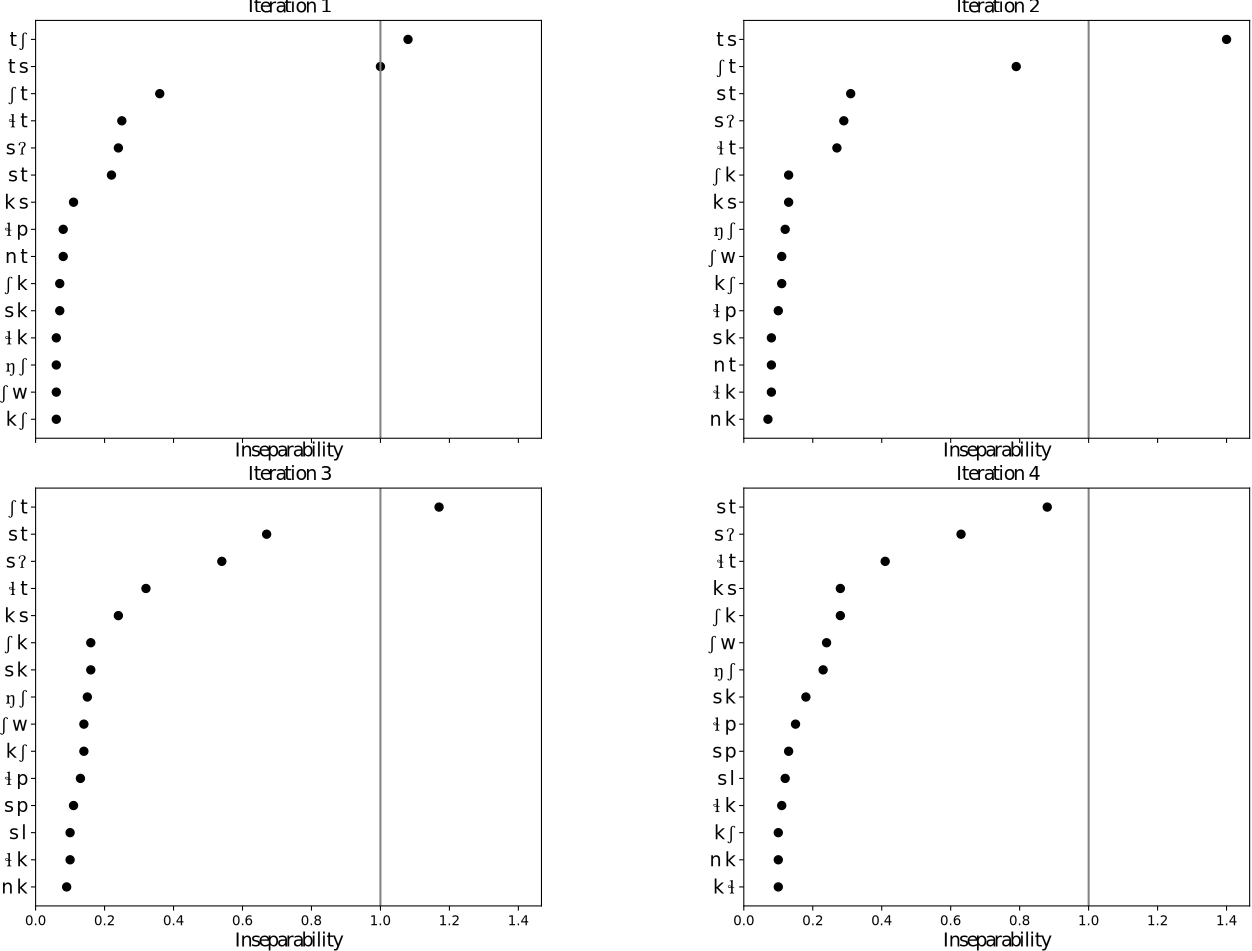
\includegraphics[width=1.0\textwidth]{figures/insepPlotsFinal.pdf}
    \caption{Plots of the inseparability value of each iteration of the complex segment learner, beginning with the first iteration in the top left, and proceeding from left to right through the remaining iterations. The vertical line indicates the threshold at which a sequence is considered to be a complex segment by the learner}
    \label{fig:insepPlot2}
\end{figure}

The output of the learner shows that affricates were established as monophonemic units by this method based on the frequency of occurrence. However, the ejective fricatives were not unified by the learner, as they occur in frequencies similar to those of other fricative + stop clusters. In later iterations, the most frequent ejective {/s'/} does approach the inseparability threshold, well ahead of any of the other ejective fricatives. This perhaps suggests that this sequence may be on its way to becoming sufficiently frequent that the learner could identify it as a complex monophonemic unit within Upper Necaxa Totonac phonology. This also illustrates the different rates at which various sequences occur in the data. Despite never crossing the threshold in the learner, the overall frequency of <s ʔ> suggests it has a different pattern from the other purported ejective fricatives. There is some potential that the shift from cluster to ejective is well underway, but only applies to the alveolar items. However, the learner also unified the sequence <{ʃ} t>, which has not been identified as a unit by linguists, in the third iteration. We can also see that the sequence <s t> was also approaching the inseparability threshold ahead of the most frequent ejective {/s'/}. This result may be due to the choice to use the \textit{Dictionary} as the data source, or may highlight the limitations of relying on segmental frequency, which may not be sufficient to establish phonemicity in all cases. The present chapter will leave the question of the suitability of dictionary data to this application for future work on the phonotactics of Upper Necaxa Totonac.

%\clearpage
\section{Phonetics of ejective fricatives in Upper Necaxa Totonac}\label{section:phonetics}
The above analyses have demonstrated that the ejective fricatives are distributed similarly to fricative + stop clusters in the lexicon. They have also shown that, at least in the \textit{Upper Necaxa Totonac Dictionary}, the ejective fricatives do not occur at sufficiently high frequencies for a computational learner to identify them as complex monophonemic units. In this section, the phonetic nature of these sequences is considered, with a focus on the acoustic duration of ejective and pulmonic fricatives. The results show that the ejectives are unlikely to be produced by the glottalic airstream, and instead fit within observed patterns of duration compatible with an analysis of them as fricative + stop clusters.

\subsection{Duration in fricative categories}\label{section:FricDur}
Production of ejective fricatives frequently involves intervals of frication preceded or followed by intervals of silence (indicating oral or glottal closure, or a lack of airflow). Comparison of the duration of these intervals to analogous intervals in pulmonic fricatives has often revealed salient differences between the airstream categories.

\subsubsection{Frication intervals}
Ejective fricatives are often found to be produced with shorter frication intervals compared to their pulmonic counterparts. In Tlingit, ejective fricatives were produced with 148 ms of frication noise compared to 222 ms in pulmonic fricatives \citep{Maddieson2001a}. Ejective fricatives in Turkish Kabardian were produced with frication intervals of about 130 ms, compared to 191 ms for pulmonic fricatives \citep{Gordon2006}. Similar patterns were also found to be the case in Mehri (88 vs. 122 ms; \citealt{Ridouane2015,Ridouane2017}) and Amharic (85 vs. 134 ms; \citealt{Demolin2002,Seid2009}). As a follow up to the measurement of frication duration in normal speech, speakers of Amharic were asked to maintain frication for as long as they could in both ejective and pulmonic conditions. The result was about 10 seconds of noise in pulmonic fricatives, and 0.6 seconds of noise in ejective fricatives. This demonstrates the limited air supply during ejective production and strengthens the description of the sounds as ejective. A notable exception to the usual finding is the pattern seen in Yapese \citep{Maddieson1998}. In this case, frication durations were roughly similar across pulmonic and ejective categories, differing by only about 20 ms at the two places of articulation studied: labiodental -- 100 vs. 120 ms, interdental -- 150 vs. 170 ms. Although they appear to be monophonemic units, the production of ejectives in Yapese involves a sequence of fricative constriction followed by glottal constriction, in other words a phonetic cluster. In Upper Necaxa Totonac, \citet{Beck2006} found that ejective fricatives were produced with 143 ms of frication noise while pulmonic fricatives were produced with only 96 ms of frication before vowels and 101 ms in fricative + stop clusters. Despite the variability of frication across languages, this is the only reported case of ejective fricatives having longer frication intervals than pulmonic fricatives. 

\subsubsection{Flanking silent intervals}
Ejective fricatives are often produced with silence preceding and/or following frication, though this varies by language and speaker. \citet{Gordon2006} report that ejective fricatives were followed frequently by a silence in Turkish Kabardian, though the duration of this silent interval was unquantified. In Mehri, some speakers were found to almost always produce silent intervals while others almost never did \citep{Ridouane2015}. In this study, pulmonic fricatives were followed by silent intervals. In ejective fricatives, the average post-frication lag interval ranged from about 21 ms word-initially to 25 ms between vowels. Intervocalic ejectives were also preceded by a silent interval of approximately 24 ms on average. In Amharic, ejective fricatives were followed by post-frication lags of approximately 30 ms \citep{Demolin2002,Seid2009}, while \citet{Maddieson2001a} found post-frication silent intervals of 46 ms in ejective fricatives and 1 ms in pulmonic fricatives in Tlingit. \citet{Beck2006} reports a post-frication silent interval of 9 ms in ejectives and 3 ms in pulmonic fricatives in Upper Necaxa Totonac.

\subsubsection{Total duration}
Comparisons of total duration tend to reveal no difference between ejective and pulmonic fricative categories \citep{Ridouane2015,Ridouane2017,Maddieson2001a}. However, ejective fricatives in Amharic were reported to have shorter duration than pulmonic fricatives in all conditions (initial and word-medial singleton fricatives, and word-medial geminate fricatives; \citealt{Seid2009}).

\subsection{Methods}\label{section:methods}
Digital audio recordings were provided by four speakers of Upper Necaxa Totonac. The audio files were annotated and segmented, and durations of various events during the production of the ejective fricatives were measured and compared. This section provides further information about the materials and methods used in the phonetic study.

\subsubsection{Speakers and Recordings}
Four speakers of Upper Necaxa Totonac (two women, two men) provided the audio data included in the acoustic analyses. Speakers ranged in age from about 30--60 years old. All speakers had grown up speaking Upper Necaxa Totonac in the area local to Patla and Chicontla, with younger speakers being exposed to more Spanish earlier in life. All of the speakers still speak Upper Necaxa Totonac in the community on a daily basis, though Spanish is also very frequently used. Interactions with the author were undertaken in Spanish.

Recordings were made in speakers' homes using a digital recorder and head-mounted microphone. The word list was presented in the same order to all speakers, though it was not intentionally arranged in any particular order. Speakers were asked to repeat each word three times within the frame sentence \textit{ixla wanli' ... chuwa} {[ʃla wanlḭ ... tʃuwa]}, meaning roughly `he said ... now'. During recording, speakers were able to see and read both the intended Upper Necaxa Totonac form and the written translations in Spanish on the author's laptop screen. In addition to these written prompts, speakers were also orally prompted with a Spanish translation.

\subsubsection{Materials}
The word list for this study was compiled from orthographic forms found in the \textit{Upper Necaxa Totonac Dictionary} \citep{Beck2011}. The list was designed to balance potential sources of variability in ejective fricatives, pulmonic fricatives, and affricates. \tabref{tab:wordsample} provides examples of words in each condition. Tokens were collected across word position, segmental context, and proximity to lexical stress. Word list items were not controlled for the number of segments that appear in the word. The  list as designed consisted of 130 words. Forms that were not produced by all speakers, including speech errors and alternative forms, were excluded from the analyses, resulting in 121 common lexical items and 1,452 fricative tokens expected to be included in the analysis. Twelve words included two different fricative tokens, increasing the overall number of expected tokens to 1,500. In some cases, speakers did not recognize the word that was intended by the word list, or produced fewer than three usable repetitions of some words, reducing the final data set to 1,430 productions.\footnote{The complete wordlist is available in \citet{Puderbaugh2019a}.}

\begin{table}[t]
%\begin{sidewaystable}
\caption[Sample lexical items by condition]{Examples of Upper Necaxa Totonac words presenting various frication conditions. Stress and laryngealization refer to the categorization of the following vowel. Target segments are shown in \textbf{bold} in orthographic representations}
\label{tab:wordsample}
\begin{tabularx}{\textwidth}{lQQQQ}
	\lsptoprule
	&\multicolumn{2}{c}{Word Initial} & \multicolumn{2}{c}{Word Medial}\\\cmidrule(lr){2-3}\cmidrule(lr){4-5}
	&{stressed}&{unstressed} &{laryng}& {non-laryng}\\\midrule
	{pulmonic} &\textit{\textbf{s}\'a:sti'} &\textit{\textbf{s}al\'un} &\textit{s\'e'h\textbf{s}i'} & \textit{ta\textbf{s}a:tan\'u:n}\\
	&{/ˈsaːs.tḭ/} &{/sa.ˈlun/} &{/ˈsḛʔ.sḭ/}&  {/ta.saː.ta.ˈnuːn/}\\
	&`new' &`hoe' &`sweet'& `stuck, fixed in place' \\\addlinespace
	{ejective} & \textit{\textbf{s'}\'a'lhwa'} &\textit{\textbf{x'}etím} &\textit{li:\textbf{lh'}\'a:'n}&\textit{ta\textbf{s'}awí} \\
	& {/ˈs'a̰{{ɬ}}.wa̰/} &{/ʃ'e.ˈtim/}&{/liː.ˈ{{ɬ}}'a̰ːn/} & {/ta.s'a.ˈwi/}\\
	&`slow of &`seeded and &`plough'&`lose, be\\
	& movement or thought' &deveined chili'&&defeated'\\
	\midrule
	{cluster} &\textit{\textbf{x}ka'j} &\textit{\textbf{lh}tak\'a'la'} &\textit{li:\textbf{x}pa't\'an} &\textit{tu:\textbf{s}p\'ulh}\\
	&{/ˈʃka̰h/}&{/{{ɬ}}ta.ˈka̰.la̰/}&{/liːʃ.pa̰.ˈtan/}&{/tuːs.ˈpu{{ɬ}}/}\\
	&`pineapple'&`board' &`pestle of &`one's toes'\\
	&&&a \textit{molcajete} &\\
	&&&(mortar)'&\\\addlinespace
	{affricate} &\textit{\textbf{ch}í'px}&\textit{\textbf{tz}al\'a'j} &\textit{chu'\textbf{ch}ó'hx}&\textit{a:'tu:'\textbf{ch}i:y\'e:tlh}\\
	&{/tʃḭpʃ/}&{/tsa.ˈla̰h/}&{/tʃṵ.ˈtʃo̰ʔʃ/}&{/a̰ː.tṵː.tʃiː.ˈjeːt{{ɬ}}/}\\
	&`dense'&`brittle, fragile, thin (stick)'&`banana blossom' &`mint'\\
	\lspbottomrule
\end{tabularx}
\end{table}

\subsubsection{Annotation}
The recorded audio was annotated to allow for consistent comparison among tokens. All instances of fricatives and affricates appearing in the data were included in the annotations and subsequent analysis, which means that some word forms containing more than one fricative contributed multiple data points per repetition. The audio files were labeled in accordance with the phonemic forms of words as transcribed in the dictionary \citep{Beck2011}, rather than the auditory impression of each segment. The segmentation and annotation was completed using Praat \citep{Boersma2018}.


 
Tokens were annotated according to three possible events: pre-frication closure, frication noise, and post-frication lag. Closure intervals were defined as beginning at the end of the second formant in the preceding vowel or sonorant, or the abrupt end of frication noise where applicable, and ending with the onset of broad spectrum energy in the release (burst or frication), or the onset of vowel phonation in cases where the release burst was not apparent. Closure intervals were labeled with the name of the following segment and <c> for closure (e.g. <tc> indicates the closure of an alveolar stop). Although all fricatives were most commonly produced without any preceding closure, some instances of pre-frication silence were observed in fricatives of both airstream types. Frication intervals began with a burst, if present, or the onset of frication noise, and ended with the end of noise, as indicated by visible amplitude in the waveform, or the onset of modal vowel phonation, where present. Frication intervals were labeled according to the segmental category (e.g. <{tʃ}> for a post-alveolar affricate, or <{ʃ'}> for a post-alveolar ejective fricative). In many tokens, frication was followed by an interval of silence or near silence before the beginning of modal phonation in the following vowels, regardless of supposed airstream mechanism. Figures \ref{fig:palvej}-\ref{fig:release} illustrate sample annotations of the data.
	

\begin{figure}[h]
    \includegraphics[width=0.6\textwidth]{figures/chaa1hO1x1a1.png}
    \caption{Post-frication silent interval in {/ʃ'/}. Detail from \textit{cha:'hó'x{'}a'} \mbox{/tʃa̰ːˈʔo̰ʃ'a̰/} `tree bark'}.
    \label{fig:palvej}
\end{figure}

\begin{figure}
	\includegraphics[width=0.6\textwidth]{figures/kilhpa1nlhU1lu1-HFM}
	\caption[Annotated spectrogram of pre-frication closure]{Pre-frication silence in {/{ɬ}/}. Detail from \textit{\textbf{kilh}pa{\textquotesingle}nlh\'ulu{\textquotesingle}} {/ki{{ɬ}}pa̰n{{ɬ}}ulṵ/} `jowly, with swollen cheeks'}
	\label{fig:closure}
	\end{figure}

\begin{figure}
	\includegraphics[width=0.6\textwidth]{figures/aa1tuu1chiiyEEklh-HFM.png}
	\caption[Annotated spectrogram of a post-alveolar affricate]{Pre-frication closure in a production of the affricate {/tʃ/}. Detail from \textit{a:{\textquotesingle}t\textbf{u:{\textquotesingle}chi:}y\'e:klh} {/a̰ːtuːtʃiːˈjeːk{{ɬ}}/} `mint'}
	\label{fig:release}
\end{figure}


\subsection{Results}\label{section:results}
This section reports descriptive statistics on the duration of frication and of silent intervals, and total duration during the production of ejective and pulmonic fricatives in various contexts. Ejective fricatives have shorter frication duration than pulmonic fricatives before vowels, but similar frication duration compared to fricatives before pulmonic stops. Clusters have longer post-frication silent intervals than ejective fricatives, but this is found to vary by place of the stop closure. Overall duration varies according to condition, with ejective fricatives and cluster having the longest durations and affricates the shortest. Further details appear below.

\subsubsection{Frication duration}
\tabref{tab:fdursummary} presents descriptive statistics for frication intervals only. Pulmonic fricatives were produced with the longest average frication duration, and affricates with the shortest. Average frication intervals of ejective fricatives and fricative + stop clusters were roughly equal. A pairwise comparison of least-squares means between all four conditions showed significant differences between all conditions ($p < 0.005$) except between ejectives and fricative + stop clusters ($\text{df} = 148.17$, $t = 1.457$, $p = 0.47$). Statistical analysis did not show any significant differences in frication duration based on place of articulation.\footnote{The statistical models on which these results are based are provided in the Appendix to this chapter. See \citet{Puderbaugh2019a} for further information on the statistical models and detailed results.}

\begin{table} 
	\caption[Frication duration in milliseconds of four phone types]{Frication duration in four phone types}
	\label{tab:fdursummary}

	\begin{tabularx}{\textwidth}{Q rrrrr}
		\lspbottomrule
		&{Mean}&{Median}&{SD}&{SE}&{\textit{N}}\\
		\midrule
		affricate\newline /t͡s, t͡ʃ/ &87 &79 &55 &4.44&151\\
		\tablevspace
		pulmonic\newline /s, ʃ, ɬ/&161 &159 &46 &3.27&196\\
		\tablevspace
		ejective\newline /s', ʃ', {ɬ}'/ &135 &130 &34 &1.38&615\\
		\tablevspace
		cluster (fricative + stop)\newline /sp, st, sk, ʃp, ʃt, ʃk, ɬp, ɬt, ɬk/ &137 &131 &37 &1.73&468\\
		\lspbottomrule
	\end{tabularx}
\end{table}

\subsubsection{Duration of post-frication silence}

\tabref{tab:lag-condition-summary} reports the duration of post-frication silent intervals across the four frication conditions. These results show that pulmonic fricatives and affricates have similar average post-frication lag times of 16 ms and 25 ms, while ejective fricatives and clusters more closely resemble each other with average lag durations of 88 ms and 123 ms. The difference in average duration in ejective fricatives and clusters is considered in more detail below.

   \begin{table}
        \centering
    	\caption[Summary of silent intervals following frication]{Duration in milliseconds of silent intervals following frication}
    	\label{tab:lag-condition-summary}

    	\begin{tabularx}{\textwidth}{Q rrrrr}
    		\lsptoprule
    		&{Mean}&{Median}&{SD}&{SE}&{\textit{N}}\\
    		\midrule
    		affricate\newline /t͡s, t͡ʃ/ &16 &15 &5 &1.15&22\\
    		\tablevspace
    		pulmonic\newline /s, ʃ, ɬ/ &26 &17 &27 &4.08&43\\
    		\tablevspace
    		ejective\newline /s', ʃ', ɬ'/ &88 &84 &39 &1.61&582\\
    		\tablevspace
    		cluster &124 &118 &42 &1.96&460\\
                (fricative + stop) \newline /sp, st, sk, ʃp, ʃt, ʃk, ɬp, ɬt, ɬk/\\
    		\lspbottomrule
    	\end{tabularx}
    \end{table}

As a follow up, items appearing in clusters (represented by the bottom row of \tabref{tab:lag-condition-summary}) were further subdivided into sets according to the place of articulation of the stop. \tabref{tab:postlag-ejclusters-summary} and \figref{fig:postfric-place} report the duration of silent intervals grouped by the place of stop closure. In both the figure and the table, ejective fricatives are referred to as having a ``glottal'' place of closure. The average closure duration was longest in bilabial closures, and shortest in glottal closures. Pairwise comparisons between these places of stop closure showed that durations differed significantly between the bilabial and glottal places ($\text{df} = 13.30$, $t = -4.482$, $p < 0.005$), and between alveolar and glottal places ($\text{df} = 6.19$, $t = -3.45$, $p < 0.05$). No other pairs differed significantly from one another.

    \begin{figure}
        \caption{Duration in milliseconds of post-frication silence in clusters and ejective fricatives. The place represented here refers to the place of closure. For ejective fricatives, this is indicated as ``glottal''}
       \includegraphics[width=0.8\textwidth]{figures/lagplace-grayscale.png}
        \label{fig:postfric-place}
    \end{figure}

    \begin{table}
        \caption[Summary of post-frication silence durations across place of closure]{Duration of post-frication silence at four places of closure in fricative + stop clusters, rounded to the nearest millisecond. Ejective fricatives are considered here as consisting of frication followed by a glottal stop closure}
    	\label{tab:postlag-ejclusters-summary}

    	\begin{tabularx}{\textwidth}{lYYYYY}
    		\lsptoprule
    		&{Mean}&{Median}&{SD}&{SE}&{\textit{N}}\\
    		\midrule
    		bilabial {/p/} &134 &131 &39 &3.68&115\\
    		alveolar {/t/} & 130& 123 &47 &3.79&155\\
    		velar {/k/} &117 &108 &35 &2.87&149\\
    		glottal /ʔ/ &88 &84 &39 &1.61&582\\
    		\lspbottomrule
    	\end{tabularx}
    \end{table}
    
\newpage
\subsubsection{Total duration}
\tabref{tab:total-dur-summary} presents descriptive statistics of the total duration (from onset of frication to onset the following vowel) in four frication conditions (affricates, pulmonic fricatives, ejective fricatives, and fricative + stop clusters). Affricates were produced with the shortest average duration, and clusters with the longest. A pairwise comparison between least-squares means of all conditions revealed that all conditions differed significantly from each other ($p < 0.005$).

\begin{table}
	\caption[Total duration in four phone types]{Total duration in four segment types, including frication and flanking silences and rounded to the nearest millisecond}
	\label{tab:total-dur-summary}

	\begin{tabularx}{\textwidth}{Qrrrrr}
		\lsptoprule
		&{Mean}&{Median}&{SD}&{SE}&{\textit{N}}\\
		\midrule
		affricate\newline /t͡s, t͡ʃ/&98 &84& 58 &4.74&151\\
		\tablevspace
		pulmonic \newline /s, ʃ, ɬ/&179 &164 &73 &5.24&196\\
		\tablevspace
		ejective\newline /s', ʃ', ɬ'/&218 &210 & 60 &2.41&615\\
		\tablevspace
		cluster (fricative + stop)\newline /sp, st, sk, ʃp, ʃt, ʃk, ɬp, ɬt, ɬk/ &260 &247 &66 &3.08&465\\
		\lspbottomrule
	\end{tabularx}
\end{table}

\subsection{Summary}
\tabref{tab:resultssummary} provides a comparison of previously reported duration data and the results of the present study. In the present study, the results show that frication intervals in the ejective fricatives of Upper Necaxa Totonac fall within the range of observed durations in other languages: frication was shorter in ejective fricatives than in pre-vocalic pulmonic fricatives and longer than in affricates. Between clusters and ejective fricatives, frication duration was nearly identical. Post-frication silent intervals were substantially longer than reported in previous work and found to vary according to the place of stop closure. As a result of the long frication and long silent intervals, ejective fricatives were found to have greater total duration than pulmonic fricatives, a finding that is again out of line with previous findings in languages with confirmed ejective fricatives. In light of this variation, the post-frication silences in ejective fricatives could be interpreted as a continuation of a general trend of shorter duration at places of articulation further back in the vocal tract. Such an interpretation would support the analysis of these sequences as clusters of segments rather than monophonemic units.

\begin{table}
    \caption{Summary of ejective fricative duration data, rounded to the nearest millisecond. Blanks indicate a lack of available data}
    \label{tab:resultssummary}
    \begin{tabularx}{0.9\textwidth}{lrrr}
		\lsptoprule
		& Frication & Silences & Total duration\\
		\midrule
		{Other languages} & (\sectref{section:FricDur})&&\\
		Pulmonic & 106--222  & & 106--223  \\
            Ejective & 120--148  & 21--45  & 88--194  \\
		\midrule
		{Upper Necaxa Totonac} & \citep{Beck2006}&& \\
		Pulmonic & 96  & 3  & \\
		Ejective & 143  & 9  & \\
		Cluster & 101  &  & \\
		Affricate &  &  &  \\
		\midrule
		{Upper Necaxa Totonac} & (\sectref{section:results})&& \\
		Pulmonic & 159--161  & 17--26  & 164--179 \\
		Ejective & 130--135  & 84--88  & 210--218 \\
		Cluster & 131--137  & 118--124  & 247--260  \\
		Affricate & 79--87  & 15--16  & 84--98 \\
        \lspbottomrule
    \end{tabularx}
%     \todo[inline]{no values for affricate?}
\end{table}

\section{Ejective fricatives or glottal stop clusters?}\label{section:discussion}

The ejective fricatives of Upper Necaxa Totonac appear at first to be quite unusual, not only because of their supposed ejectivity but also because of the structure of the consonantal system they are a part of. In order to be \textit{rare}, however, we must first determine that they are in fact what we claim them to be. The phonology of Upper Necaxa Totonac gives no immediate clues to the monophonemic status of ejective fricatives. The ejective fricatives in Upper Necaxa Totonac are far less common than the pulmonic fricatives across all places of articulation. They are limited only to onset position and are presumed not to resyllabify the way that fricative + stop clusters do. In their distributions, they seem at first to resemble affricates, which are similarly limited in where they may occur. However, unlike the affricates ejective fricatives appear to be quite rare even in their limited environments, posing challenges to their potential learnability. However, when we compare the ejective fricatives to fricative + glottal stop clusters, we see that they occur at frequencies similar to the other combinations, with the exception of alveolar clusters, which are all but nonexistent in the data. This finding of parallelism between the ejective fricatives and fricative + stop clusters is not surprising given the historical shift from *q in Proto-Totonacan to /ʔ/ in Upper Necaxa Totonac. The overall duration of the ejective fricatives also aligns well with an interpretation of them as clusters. Where previous studies of ejective fricatives in other languages have found that the overall duration of pulmonic and ejective fricatives are similar to one another, the ejective fricatives of Upper Necaxa Totonac are instead longer than their pulmonic counterparts in the present findings. The small differences in total duration that do appear seem to be related to the place of closure during stop production, rather than to a unique production mechanism during frication. These findings are substantively different from those reported by \citet{Beck2006}, who found instead that the pulmonic fricatives had frication periods shorter than any other reported language, as well as shorter than that of the ejective fricatives.

There are two options for analysis here: ejective fricatives are phonemically ejective, contrasting with pulmonic fricatives, or ejective fricatives are clusters among an established series of fricative + stop clusters. There are no clear-cut criteria for answering this question, despite proposals for possible ways of distinguishing these categories extending back into the early 20th century \citep{Trubetzkoy1939,Pike1947,Stark1947,Uchihara2021}. According to Trubetzkoy's criteria, in order to postulate a unit phoneme, (i) sequences may not break over a syllable boundary; (ii) complex articulations must be homorganic; (iii) the combined duration may not exceed that of other phonemes in the same language; (iv) sequences may appear in positions where clusters are not allowed; (v) the analysis of complex sounds must lead to symmetry in the phonemic inventory; (vi) the constituent parts of the sequence may not be interpreted as allophones of other phonemes. 

The ejective fricatives of Upper Necaxa Totonac do not break over syllable boundaries, but their component articulations are not homorganic. The overall duration of the ejective fricatives is longer than that of any other unit phonemes, and similar to that of clusters. The ejectives appear in precisely the same locations as clusters, particularly if we consider the /ʔ/ + fricative coda clusters to be the mirror image of ejective fricatives. The inclusion of ejective fricatives in the Upper Necaxa Totonac sound inventory introduces an odd asymmetry by requiring a production mechanism that is not used for any more common purpose in the sound system. It is furthermore possible that only one (alveolar) of the three purported places of articulation is currently developing toward a coalescence of its component parts, which would lead to further asymmetry. Neither the fricatives nor the glottal constriction are unique to the ejective fricatives. Thus, on most of these criteria, the ejective fricatives do not seem to be instances of complex segments, but rather clusters.

Another potential set of criteria for determining whether sequences should be interpreted as units or clusters is provided by \citet{Pike1947}. In addition to tautosyllabicity, which has already been addressed above, Pike posits two criteria: (i) parallel patterns in straightforward sequences can be held as evidence for those that are in question; (ii) sequences that are paralleled by the reverse of the same segments ought to be interpreted as clusters. The data and analysis in \sectref{section:collocation} have shown that the ejective fricatives are paralleled by many straightforward sequences of fricatives in combination with various other stops. The data also show that the ejective fricatives are mirrored by sequences of /ʔ/ + fricatives sequences in coda position. Thus, besides appearing tautosyllabically, which is in fact an empirical question that has not been thoroughly addressed, the ejective fricatives of Upper Necaxa Totonac also fail to meet most of Pike's criteria for complex segments.

We can compare the above considerations to a similar scenario relating to the affricates {/t͡s, t͡ʃ/}. These segments do not break over a syllable boundary. In fact, clusters of {/t/} and {/s/} or /ʃ/ do not even occur in environments that might potentially lead to ambiguity on this point. Both {/t͡s, t͡ʃ/} are homorganic articulations. The overall duration of these complex units is shorter than any fricatives or clusters. They do appear where other clusters are not allowed in that stop + fricative sequences are limited to coda position, while the affricates appear only in onset position. Their inclusion in the sound inventory does not introduce any asymmetry. Their constituent parts do appear as allophones of other phonemes. Furthermore, the affricate sequences are not paralleled by similar combinations of stops followed by frication. While they are not paralleled by their reverse sequence in coda position, {/st/} and {/ʃt/} do appear in syllable onsets. Thus, the affricate phonemes of Upper Necaxa Totonac satisfy five of Trubetzkoy's six criteria, and largely also conform for to Pike's two criteria. On balance, the affricates appear to be well analyzed as monophonemic rather than clusters, unlike the ejective fricatives.

\section{Conclusion}
The data and analyses above have shown that there are many reasons to believe that the ejective fricatives of Upper Necaxa Totonac are in fact fricative + glottal stop clusters. The data show that they more closely resemble clusters than other complex segments in the language, and they fail to meet most classical criteria for determining complex segmenthood. They furthermore fail tests of learnability with modern computational methods, and their acoustic durations also suggest that they are in fact clusters. Interestingly, although the data indicates that they are not ejective, fricative + glottal stop clusters are themselves rather rare and therefore of potential interest for phonological typology. 

The current puzzle is an example of a common problem in phonological typology: the source and veracity of available documentation. The set of implicit criteria used for determining segmenthood in descriptive and documentary contexts is not at all well delimited. However, it is crucial to the identification of any phonological universals or rarities that we establish transparent and thorough methods for relating the two fields. Both phonetic and phonological evidence need to be taken into account when determining the identity of particular sounds used in language. The identification of ejective fricatives in Upper Necaxa Totonac was based primarily on the impressions of an individual linguist that were integrated into the \textit{Upper Necaxa Totonac Dictionary} \citep{Beck2011}. When considering the phonological typology, we must ensure that we are talking about well-established phonological entities with clear evidence behind them. If the ejective fricatives are monophonemic, the sound system of Upper Necaxa Totonac is a typological oddity. On the other hand, if they are clusters, the synchronic phonology of Upper Necaxa Totonac becomes much simpler, with clear and common historical changes leading to its present configuration. This second scenario aligns with the phonetic data presented here. It is furthermore in line with the general phonotactic patterns of the language, which allow for fricative + stop clusters in every environment where ejective fricatives also occur. Interpreting the ejective fricatives as clusters would therefore simplify the segmental inventory of Upper Necaxa Totonac and eliminate the need to explicate the rarity. Because databases that are used to investigate phonological typology and phonological universals tend to include information relating only to individual segmental contrasts, it is difficult to say whether clusters of fricatives and glottal stops constitute phonological rarities themselves. In the absence of either phonetic or phonological evidence for a unique segmental contrast, perhaps it is best to consider the alternative analytical solutions which will make it not so rare after all.

% \section*{Abbreviations}
% \begin{tabularx}{.8\textwidth}{@{}lQ@{}}
% ... & \\
% ... & \\
% \end{tabularx}%
% \begin{tabularx}{.8\textwidth}{@{}lQ@{}}
% ... & \\
% ... & \\
% \end{tabularx}

\section*{Acknowledgements}
Portions of this research were previously presented in \citet{Puderbaugh2015}, \citet{Puderbaugh2019a}, and \citet{Puderbaugh2019}. The data presented here was collected on field trips supported by a travel grant from the Jacobs Research Fund at the Whatcom Museum in Bellingham, WA, and a grant from the Social Sciences and Humanities Research Council awarded to Dr. David Beck at the University of Alberta.

\section*{Appendix}\label{section:Appendix}
This section presents summaries of the models used in the statistical analysis of \sectref{section:FricDur}. The models were built separately for each dependent variable. In each model, the fitting procedure began with random intercepts specified for Word and Speaker to account for inherent differences between speakers and lexical items. The fixed effects structure included two-way interactions between all pairings of the independent variables (reference levels in italics): condition (\emph{ejective}, cluster, pulmonic, or affricate), word position (\emph{initial} or medial), place of articulation (\emph{alveolar}, post-alveolar, or lateral), stress (of the following vowel; \emph{unstressed} or stressed), and vowel laryngealization (of the following vowel; \emph{no} or yes). After model fitting and model criticism were complete, multiple comparisons of conditional means were performed using the \textit{lsmeans} package \citep{Lenth2016}. Further details can be found in \citet{Puderbaugh2019a}.

	%latex.default(coef_frication, file = "")%
	\begin{table}
		\caption{Summary of linear mixed effects regression model of frication duration (\textit{N} = 1,430)}\label{Table:fricdurstats}
		\footnotesize\tabcolsep=.666\tabcolsep
		\begin{tabular}{lrrrrr@{\,}l}
			\lsptoprule
			\multicolumn{1}{l}{coef} & 
			\multicolumn{1}{c}{Est.} &
			\multicolumn{1}{c}{SE} & 
			\multicolumn{1}{c}{df} & 
			\multicolumn{1}{c}{$t$} & 
			\multicolumn{2}{c}{$\text{Pr}(>|t|)$}\\
			\midrule
			(Intercept)&$ 4.9672$&$0.0740$&$  4.9433$&$67.0861$&$0.0000$&***\\
			conditioncluster&$-0.0152$&$0.0437$&$136.3694$&$-0.3481$&$0.7283$&\\
			conditionpulmonic&$ 0.0562$&$0.0522$&$225.2882$&$ 1.0752$&$0.2835$&\\
			conditionaffricate&$-0.5560$&$0.0560$&$262.1392$&$-9.9350$&$0.0000$&***\\
			v2laryngealyes&$-0.0941$&$0.0410$&$ 24.1915$&$-2.2921$&$0.0309$&*\\
			v2stressstressed&$ 0.1582$&$0.0367$&$146.3012$&$ 4.3149$&$0.0000$&***\\
			wordposmedial&$-0.1269$&$0.0552$&$  7.2171$&$-2.3005$&$0.0539$&*\\
			placepostalveolar&$-0.1026$&$0.0311$&$240.4922$&$-3.3037$&$0.0011$&**\\
			placelateral&$-0.0749$&$0.0335$&$211.5120$&$-2.2353$&$0.0264$&*\\
			conditioncluster:v2laryngealyes&$ 0.0428$&$0.0390$&$490.2559$&$ 1.0990$&$0.2723$&\\
			conditionpulmonic:v2laryngealyes&$ 0.1516$&$0.0534$&$438.6484$&$ 2.8383$&$0.0047$&**\\
			conditionaffricate:v2laryngealyes&$-0.0458$&$0.0567$&$654.4760$&$-0.8077$&$0.4196$&\\
			conditioncluster:v2stressstressed&$-0.0631$&$0.0503$&$244.9984$&$-1.2543$&$0.2109$&\\
			conditionpulmonic:v2stressstressed&$-0.0009$&$0.0741$&$154.8787$&$-0.0117$&$0.9907$&\\
			conditionaffricate:v2stressstressed&$-0.2871$&$0.0677$&$452.4925$&$-4.2419$&$0.0000$&***\\
			conditioncluster:wordposmedial&$-0.0239$&$0.0502$&$166.8000$&$-0.4748$&$0.6356$&\\
			conditionpulmonic:wordposmedial&$ 0.0603$&$0.0616$&$177.9500$&$ 0.9792$&$0.3288$&\\
			conditionaffricate:wordposmedial&$ 0.4576$&$0.0713$&$311.3013$&$ 6.4141$&$0.0000$&***\\
			v2laryngealyes:placepostalveolar&$ 0.1852$&$0.0412$&$411.2193$&$ 4.4943$&$0.0000$&***\\
			v2laryngealyes:placelateral&$ 0.1139$&$0.0458$&$473.6831$&$ 2.4881$&$0.0132$&*\\
			\lspbottomrule
		\end{tabular}
	\end{table}

	%latex.default(coef_lag, file = "")%
	\begin{table}
		\caption{Summary of linear mixed effects regression model of lag duration including all four conditions (\textit{N} = 1,107)}
		\label{Table:4condition-lag}
		\footnotesize\tabcolsep=.666\tabcolsep
		\begin{tabular}{lrrrrr@{\,}l}
			\lsptoprule
			\multicolumn{1}{l}{coef} & 
			\multicolumn{1}{c}{Est.} &
			\multicolumn{1}{c}{SE} & 
			\multicolumn{1}{c}{df} & 
			\multicolumn{1}{c}{$t$} & 
			\multicolumn{2}{c}{$\text{Pr}(>|t|)$}\\
			\midrule
    			(Intercept)&$ 4.5332$&$0.0878$&$ 10.9339$&$ 51.6322$&$0.0000$&***\\
    			conditioncluster&$ 0.3402$&$0.0805$&$  6.5995$&$  4.2252$&$0.0045$&**\\
    			conditionpulmonic&$-1.2863$&$0.2167$&$  3.8357$&$ -5.9356$&$0.0046$&**\\
    			conditionaffricate&$-1.5736$&$0.1443$&$  3.9165$&$-10.9087$&$0.0004$&***\\
    			fricationplacepostalveolar&$-0.1036$&$0.0738$&$163.9262$&$ -1.4037$&$0.1623$&\\
    			fricationplacelateral&$ 0.0935$&$0.0827$&$106.3854$&$  1.1303$&$0.2609$&\\
    			wordposmedial&$-0.3994$&$0.0846$&$ 69.9077$&$ -4.7204$&$0.0000$&***\\
    			v2stressstressed&$-0.0400$&$0.0998$&$ 13.7680$&$ -0.4012$&$0.6944$&\\
    			v2laryngealyes&$-0.0843$&$0.0351$&$402.9234$&$ -2.4028$&$0.0167$&*\\
    			fricationplacepostalveolar:wordposmedial&$ 0.3375$&$0.1100$&$138.0113$&$  3.0697$&$0.0026$&**\\
    			fricationplacelateral:wordposmedial&$ 0.1877$&$0.1162$&$128.6923$&$  1.6151$&$0.1087$&\\
    			fricationplacepostalveolar:v2stressstressed&$-0.2256$&$0.1077$&$273.3722$&$ -2.0947$&$0.0371$&*\\
    			fricationplacelateral:v2stressstressed&$-0.1326$&$0.1052$&$227.2147$&$ -1.2605$&$0.2088$&\\
    			wordposmedial:v2stressstressed&$ 0.3929$&$0.1014$&$209.4187$&$  3.8760$&$0.0001$&***\\
    			\lspbottomrule
    		\end{tabular}
    	\end{table}

    %latex.default(coef_total, file = "")%
    \begin{table}
    \caption{Summary of linear mixed effects regression model of total duration from onset of frication to onset of following vowel (\textit{N} = 1,427)}
    \label{Table:total-dur-model}
    \footnotesize\tabcolsep=.666\tabcolsep
    \begin{tabular}{lrrrrr@{\,}l}
			\lsptoprule
			\multicolumn{1}{l}{coef} & 
			\multicolumn{1}{c}{Est.} &
			\multicolumn{1}{c}{SE} & 
			\multicolumn{1}{c}{df} & 
			\multicolumn{1}{c}{$t$} & 
			\multicolumn{2}{c}{$\text{Pr}(>|t|)$}\\
			\midrule
    (Intercept)&$ 5.4677$&$0.0702$&$  6.8185$&$ 77.8802$&$0.0000$&***\\
    conditioncluster&$ 0.1438$&$0.0517$&$120.4509$&$  2.7797$&$0.0063$&**\\
    conditionpulmonic&$-0.3024$&$0.0598$&$217.4712$&$ -5.0608$&$0.0000$&***\\
	conditionaffricate&$-0.7603$&$0.0632$&$245.0148$&$-12.0260$&$0.0000$&***\\
	v2laryngealyes&$-0.1254$&$0.0381$&$527.3923$&$ -3.2951$&$0.0010$&**\\
	v2stressstressed&$ 0.1994$&$0.0430$&$136.0534$&$  4.6328$&$0.0000$&***\\
	wordposmedial&$-0.1259$&$0.0627$&$  8.4812$&$ -2.0085$&$0.0774$&\\
	placepostalveolar&$-0.1460$&$0.0407$&$ 28.0098$&$ -3.5879$&$0.0013$&**\\
	placelateral&$-0.0847$&$0.0395$&$113.6976$&$ -2.1435$&$0.0342$&*\\
	conditioncluster:v2laryngealyes&$ 0.0882$&$0.0429$&$578.6095$&$  2.0535$&$0.0405$&*\\
	conditionpulmonic:v2laryngealyes&$ 0.2035$&$0.0591$&$492.7427$&$  3.4456$&$0.0006$&***\\
	conditionaffricate:v2laryngealyes&$-0.1106$&$0.0612$&$742.6632$&$ -1.8074$&$0.0711$&\\
	conditioncluster:v2stressstressed&$-0.1453$&$0.0575$&$230.5044$&$ -2.5291$&$0.0121$&*\\
	conditionpulmonic:v2stressstressed&$-0.1921$&$0.0870$&$143.5211$&$ -2.2082$&$0.0288$&*\\
	conditionaffricate:v2stressstressed&$-0.4729$&$0.0743$&$403.3724$&$ -6.3671$&$0.0000$&***\\
	conditioncluster:wordposmedial&$ 0.0017$&$0.0592$&$148.7945$&$0.0287$&$0.9771$&\\
	conditionpulmonic:wordposmedial&$-0.0507$&$0.0718$&$164.9282$&$ -0.7063$&$0.4810$&\\
	conditionaffricate:wordposmedial&$ 0.1060$&$0.0801$&$274.9668$&$  1.3234$&$0.1868$&\\
	v2laryngealyes:placepostalveolar&$ 0.1854$&$0.0455$&$474.7367$&$  4.0715$&$0.0001$&***\\
	v2laryngealyes:placelateral&$ 0.1066$&$0.0502$&$565.1744$&$  2.1219$&$0.0343$&*\\
	\lspbottomrule
\end{tabular}
\end{table}

\printbibliography[heading=subbibliography,notkeyword=this]
\end{document}
